%********************************************************************
% Appendix
%*******************************************************
% If problems with the headers: get headings in appendix etc. right
%\markboth{\spacedlowsmallcaps{Appendix}}{\spacedlowsmallcaps{Appendix}}
\chapter{\texttt{Modelica} \acsfont{HHPS} Model Breakdown} \label{appx:modelbreakdown}

\cref{fig:boilerandhp} shows the section of the model with many components relating to the boiler, \ac{HP}, various control related blocks and the composite block containing the reference home. The \texttt{building} block on the left connects the \texttt{.idf}-file and \texttt{.epw}-file to the \texttt{Modelica} model via \texttt{Spawn of EnergyPlus}, acting as the interface between the two softwares. the \texttt{weaBus} block directly to the right of the \texttt{building} block is the weather bus block, essentially allowing weather data to be passed to other blocks. The \texttt{bou[]} block and the block directly beneath it act as boundary condition blocks, converting the climatic data to infiltrating and exiting air to the conditioned zones. The \texttt{pumBOi} and \texttt{pumRad} blocks are the two pumps of the hydronic system. the \texttt{boi} block towards the bottom left is the boiler block described in \cref{subsec:boi}. The \texttt{tan} block bottom center is the tank model described in \cref{subsec:tank}. The various \texttt{temSup}, \texttt{temRet}, \texttt{tanTemTop}, \texttt{tankTemBot}, \texttt{temPostHP} and \texttt{tempPreHP} block are water temperature sensors. The information from the sensors are used in the control system. The \texttt{swi} blocks are logical switches. The \texttt{heaChaBoi} and \texttt{heaChaHP} blocks are the blocks which compute the supply temperature for the radiators using the curves from \cref{fig:supplytempcurves}. The various \texttt{splVal} blocks are splitting valves. The block directly left of the \texttt{splVal} block is a controllable three way splitter, being controlled by the PI-controller block \texttt{conVal}, the output of which is determined by the \texttt{temSup} sensor, and the \texttt{swi3} block (which switches between the two demand curves depending on outdoor conditions, as per the \texttt{greaterOut} block). The \HP model block is located bottom centre, directly next to the \texttt{TReturn} boundary condition block.
\begin{figure}[htb]
    \centering
    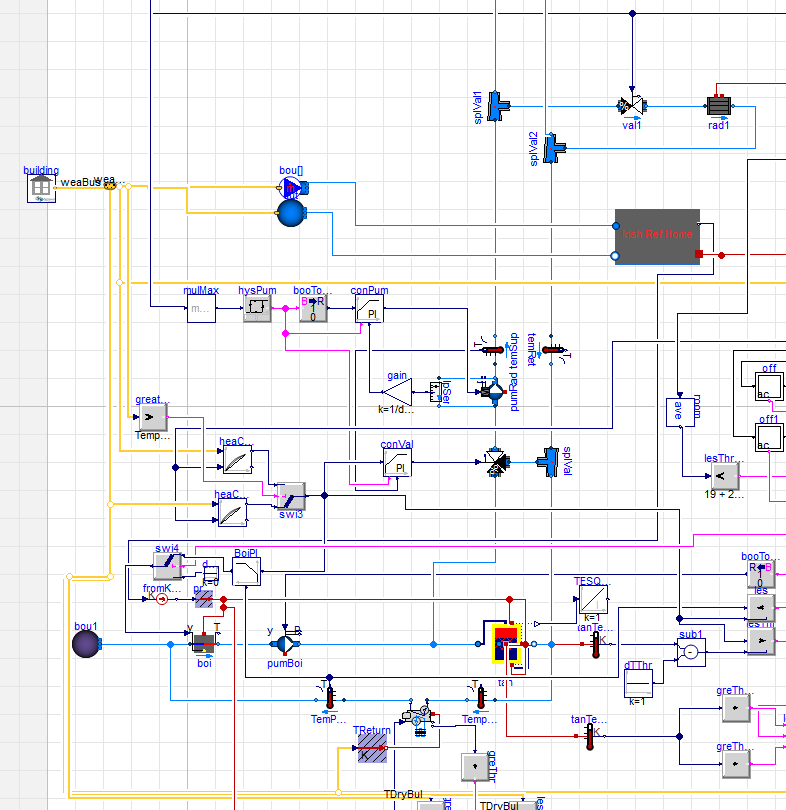
\includegraphics[width=0.9\linewidth]{boilerandHP}
    \caption{Boiler and \acs{HP} section of the \texttt{Modelica} model}
    \label{fig:boilerandhp}
\end{figure}

In \cref{fig:controllersec}, just north of the centre is the day-night setback control section. The \texttt{TRooSet} and \texttt{TRooNig} constant integer outputs are switched by the \texttt{occSch} and \texttt{swi1} blocks. This feeds into the supply temperature demand block. In the centre of the figure is the state machine portion of the control system, comprised of the various \texttt{pumOn} step blocks and \texttt{T1}, \texttt{T2}, etc. transition blocks. The top loop control the boiler and the bottom one controls the \HP. The \texttt{stateGraphRoot} block on the right is necessary for \texttt{Modelica} to keep track of the state machine. There are many \texttt{and} and \texttt{or} blocks connected to the inputs and outputs of the \texttt{Modelica.StateGraph.StepWithSignal} blocks. In the bottom centre two blocks connected by yellow lines can be seen, these are the inequality blocks to test for the outdoor temperature to block the boiler or \HP by blocking the \texttt{T3} and \texttt{T5} respectively. The \texttt{room} \texttt{Buildings.Utilities.Math.Average} block takes the temperatures of all conditioned rooms as a vector and calculates the average, and allows the \texttt{T1} and \texttt{T8} transition blocks to be unblocked if the \texttt{lesThr} block is outputting true. This block is testing whether the temperature at the top of the buffer tank is less than the demanded supply temperature. 
\begin{figure}[htb]
    \centering
    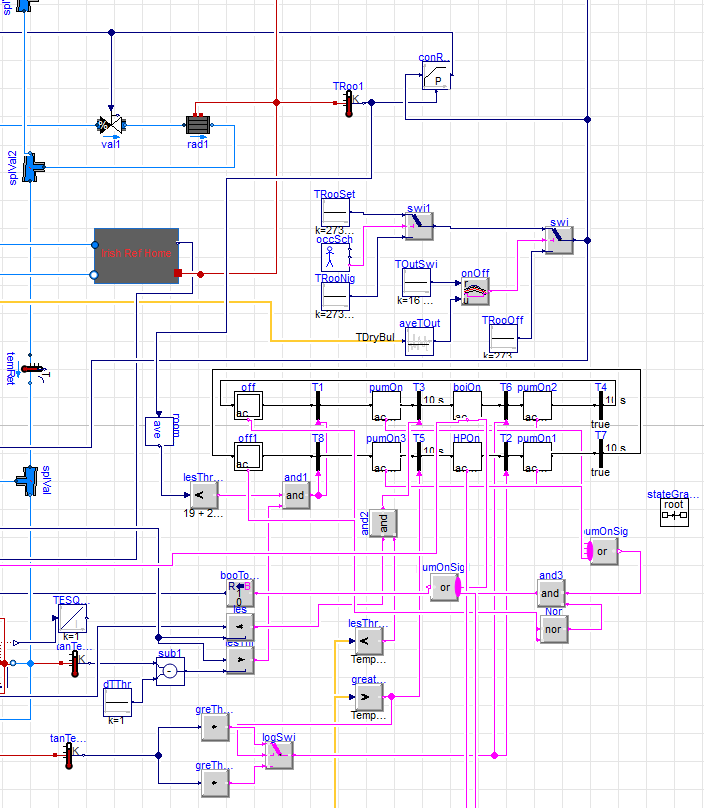
\includegraphics[width=0.9\linewidth]{controller}
    \caption{Controller section of the \texttt{Modelica} model}
    \label{fig:controllersec}
\end{figure}

\cref{fig:frostingmodelsec} shows the frosting model diagram. The \texttt{greThr} block tests whether the \HP is on, and the \texttt{lesThr1} block tests whether it outdoor temperature is less than \qty{2}{\celsius}, the output of these is put into the \texttt{and4} logical and block and passed to the \texttt{accTim} time accumulating block. It is reset if the \texttt{greThr1} block activates the threshold of the \texttt{tim} timer block after a five-minute contiguous period with $T_\text{ext}>\qty{4}{\celsius}$. The \texttt{truHol} block serves as the blocking mechanism of the \HP for a ten-minute period. The second pump and boiler models are to imitate the boiler acting in reverse, the energy usage of the \texttt{boi1} model is summed with the primary boiler model to account for the energy loss due to defrosting. 
\begin{figure}[htb]
    \centering
    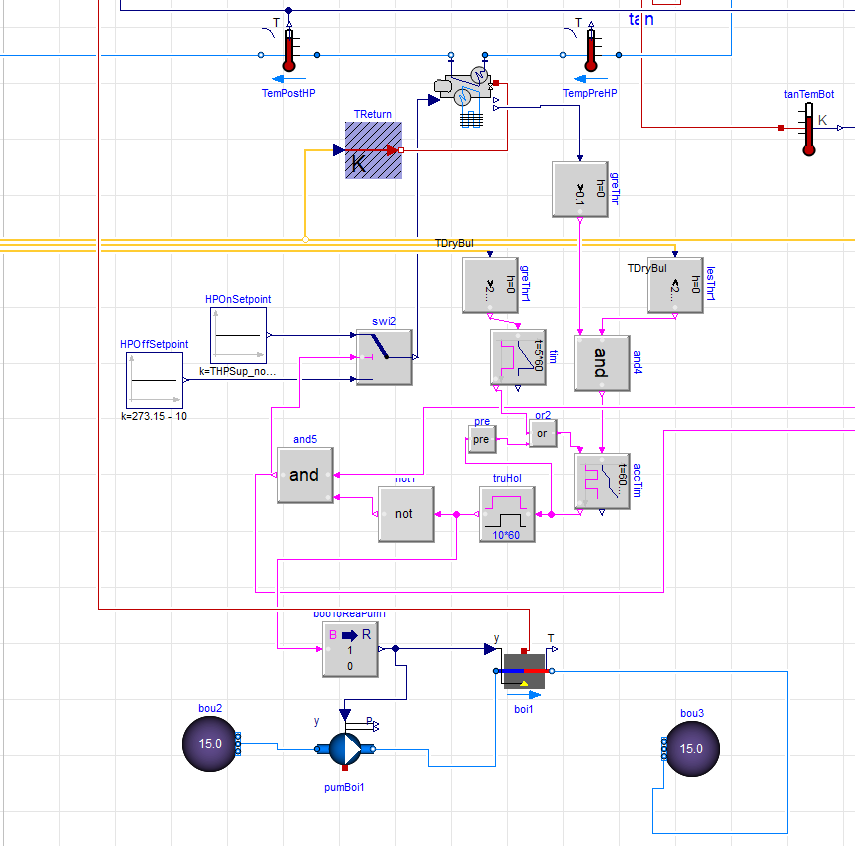
\includegraphics[width=0.9\linewidth]{frosting}
    \caption{Frosting model section of the \texttt{Modelica} model}
    \label{fig:frostingmodelsec}
\end{figure}

\cref{fig:radssec} shows the radiator section of the model. Not all of the connections are rendered as they were not created using the \texttt{Dymola} interface, rather, they were manually created in the underlying code in order to avoid mistakes. The \texttt{rad1}, \texttt{rad2}, etc. blocks are the radiator blocks, as described in \cref{subsec:rad}, serving each of the twelve conditioned rooms, with \texttt{rad3} omitted as the third indexed room is unconditioned. The \texttt{val1}, \texttt{val2}, etc. blocks are controllable valves, limiting the flowrate as a function of the respective volume of the room to the total room volume, and are controlled by the \texttt{conRoo1}, \texttt{conRoo2}, etc. P-controller blocks. The P-controllers take the respective temperature of the room as input via \texttt{TRoo1}, \texttt{TRoo2}, etc. and the \texttt{swi} block from the day-night setback switch. The output of these P-controllers feeds into the \texttt{mulMax} block from \cref{fig:boilerandhp}.
\begin{figure}[htb]
    \centering
    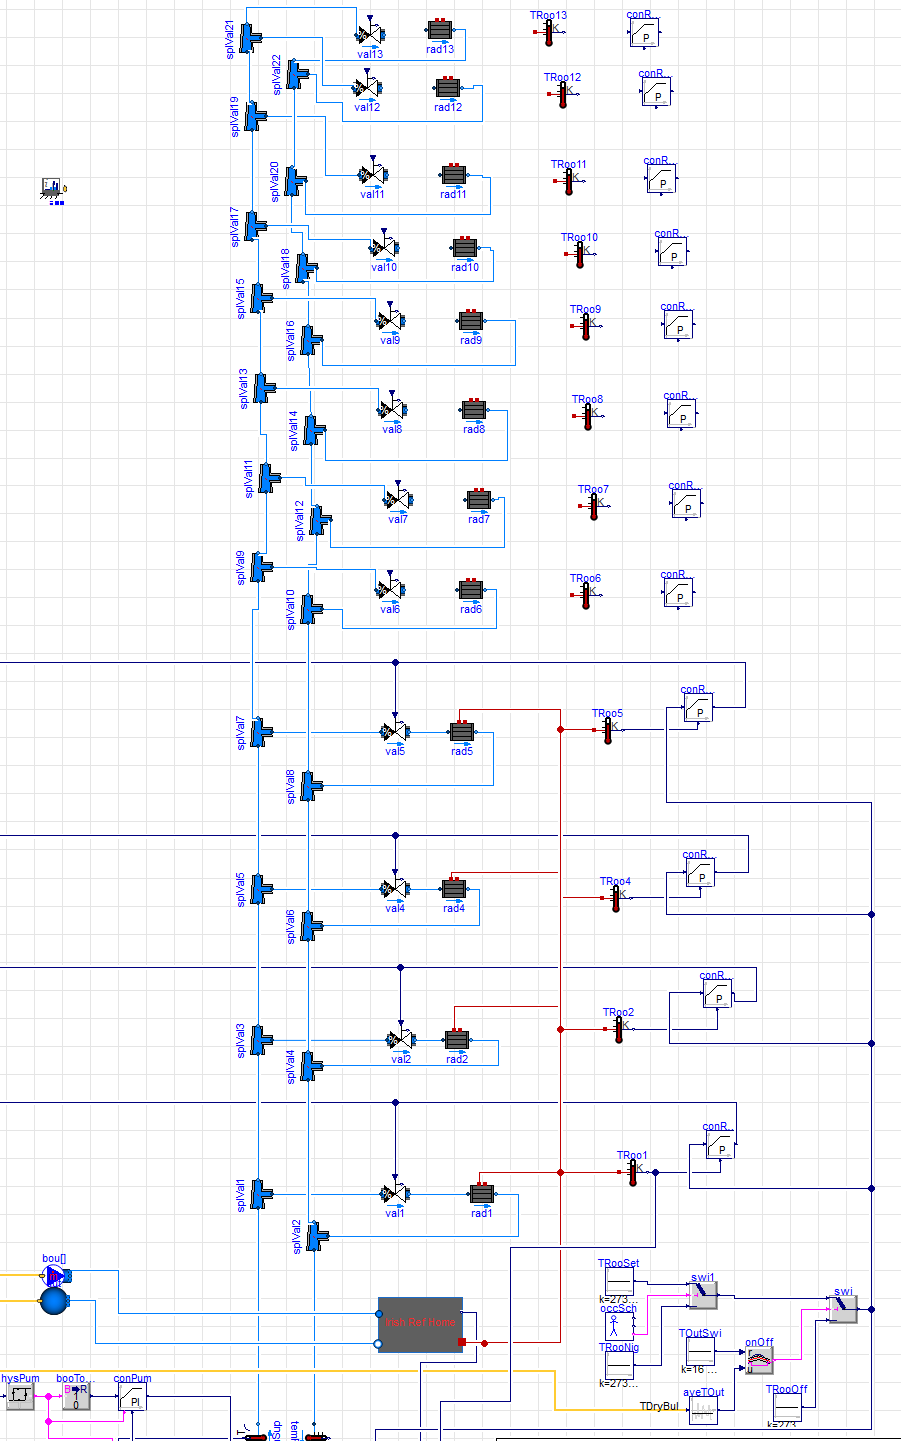
\includegraphics[width=0.85\linewidth]{rads}
    \caption{Radiator section of the \texttt{Modelica} model}
    \label{fig:radssec}
\end{figure}